%\section{Problem Description}
\section{Why Wollok?}
\label{sec:problem}

% Context, exposed with the \textbf{most precise terms possible} (don't open unwanted doors for the reader)
% Probably set the vocabulary before to cut any misinterpretation

%En la misma dirección, propongo una sección 2 bien cortita, donde nos limitemos a señalar los aspectos que apoyan lo que vamos a decir de Wollok. Y tal vez no todos, contar solamente 
%- lo del primer programa. Sobre esto, me gustaría reforzar que este programa de OO no tiene nada, con lo cual estamos desviando el foco. Se puede meter la clase Golondrina, y un main que cree una golondrina, la haga comer, y le pregunte la energía. Y fijate todo lo que hay que hacer para tener un primer ejemplo "posta-OO". Incluiría en la lista a la consola, porque no haría ejemplos con consola en Wollok.
% Los cursos se enfocan en sintaxis y usan lenguajes inadecuados.
One cause behind the difficulties in learning OOP is the use of industrial languages, which require the student to understand several concepts before being able to run his first program \cite{kolling_problem_1999}.
% Ejemplo con Java.
Figure \ref{fig:helloWorld} shows an example of a possible first program, written in Java \cite{arnold_java_1996}.
To get this program running, the student has to walk through a minefield of complex concepts: packages, classes, scoping, types, arrays, printing to standard output and class methods 
before being able to have a first object and send a message to it.

\vspace{-3mm}
\begin{figure}[ht]
 \centering
 \begin{lstlisting}[language=Java]
	package examples;
	
	public class Accumulator {
		private int total = 0;
		
		public int getCurrentTotal() { return total; }
		public void add(amount) { total += amount; }

		public static void main(String[] args) {
			Accumulator accum = new Accumulator();
			accum.add(2);
			accum.add(5);
			accum.add(8);
			System.out.println(accum.getCurrentTotal());
		}
	}\end{lstlisting}
\vspace{-3mm}
\caption{Sample initial Java program which diverts student attention from the most important concepts.}
\label{fig:helloWorld}
\end{figure}
\vspace{-3mm}

%- en particular, el ruido que le hace a los alumnos arrancar con clases.
% TODO, no estoy seguro de cómo encararlo ni de si es lo más importante.

% Por eso los pibes no aprenden
%- la tensión entre que te vaya bien en la materia y el uso de las ideas en la industria.
Courses tend to spend too much time concentrated on the details of programming constructs of a specific language, leaving too little time to become fluent on the distinctive characteristics of OOP. 
such as identifying objects and their knowledge \emph{relationships}, assigning \emph{responsibilities} 
and taking advantage of \emph{encapsulation} and \emph{polymorphism} to make programs more robust and extensible.

% Además necesitamos environments
Moreover, frequently the students do not have proper tools that could help them to overcome all the obstacles.
This might not be a problem for other introductory courses focused on the development of algorithms in procedural or functional languages, 
but it has a significative importance for object-oriented courses where we want to deal with larger programs in multiple files and to teach concepts such as testing, debugging and code reuse~\cite{kolling_problem_1999}. 

\medskip


\label{sec:wollokLanguage}

% Free form, variable number of sections, technical details.
% But in general do not mix solution and discussions/possible variation let that for discussion

Wollok provides an extremely simple programming model which allows the students to create programs containing objects, 
messages and polymorphism without the need for more abstract concepts such as classes, inheritance or type annotations.
Later in the course, Wollok allows the incremental introduction of more abstract concepts,
providing a smooth transition into a full-fledged OO programming model.

The example in Figure \ref{fig:helloWorld/wollok} shows an example first program in a Wollok-based OO introductory course.
Syntax has been reduced to a minimum and the basic constructs of the language match exactly the concepts we want to transmit, \eg \code{var} is used to define variables and \code{method} is used to define methods.
The \code{accumulator} object is defined as a stand-alone (\ie it has no visible class), automatically instantiated and \emph{well-known} (\ie globally accesible) object (WKO).
%This is also consistent with some modern industrial OO languages that allow to define both classes or standalone objects, such as Scala \cite{Oder04a}.
%To build this first program students are not required to know about typing, scoping or packaging.
%The concepts required to understand this program are no more than program, object, message and argument passing.

\vspace{-3mm}
\begin{figure}[ht]
 \centering
 \begin{lstlisting}[language=Wollok]
	object accumulator {
		var total = 0
		var evens = 0
		
		method getCurrentTotal() { return total }
		method add(amount) { 
			total += amount 
			if (amount % 2 == 0) { evens += 1 }
		}
		method evenCount() { return evens }
	}\end{lstlisting}
\vspace{-3mm}
\caption{\small Sample initial Wollok object definition.}
\label{fig:helloWorld/wollok}
\end{figure}
\vspace{-3mm}

Normally, writing to standard output as it is shown in Figure \ref{fig:helloWorld} will be considered a problem in industrial software construction.
Therefore, teaching the students to try out their programs in this way is introducing a bad practice that will have to be \emph{unlearned} later.
While some kind of user interaction is required in order to see the behaviour of our programs, proper handling of user interaction is beyond the scope of an initial OO course.

To avoid I/O a \emph{read-eval-print-loop}~(REPL) is provided.
Running a program in the REPL brings all defined objects to life and allows the user to interact with them sending messages. 
The REPL handles all I/O and the student is only required to write the desired messages to a \emph{domain object} (\cf Fig. \ref{fig:repl}).

\vspace{-3mm}
\begin{figure}[ht]
 \centering
 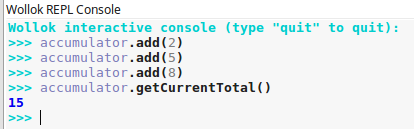
\includegraphics[scale=0.55]{images/accumulator-repl.png}
\vspace{-3mm}
\caption{\small Sample usage of the accumulator object in the REPL}
\label{fig:repl}
\end{figure}

Shortly after in the course, we introduce unit testing, 
which slowly replaces the REPL as the main form of interacting with objects. 
The Wollok test runner simplifies unit test creation for for begginners by automatically providing \emph{test isolation} \cite{martin2008cleanCode},
\ie global state is reset after each individual test case is run.
For example, the messages sent to the accumulator in the first test in Figure \ref{fig:test} will not affect the state of the accumulator in the second test.

\vspace{-3mm}
\begin{figure}[ht]
 \centering
 \begin{lstlisting}[language=Wollok]
 	import accumulator.*

	test "adding 2+5+8 should give 15" {
		accumulator.add(2)
		accumulator.add(5)
		accumulator.add(8)
		assert.equals(15, accumulator.getCurrentTotal())		
	}
   
	test "accumulator starts with 0" {
		assert.equals(0, accumulator.getCurrentTotal())
	}\end{lstlisting}
\vspace{-3mm}
\caption{\small Sample test Wollok program.}
\label{fig:test}
\end{figure}
\vspace{-3mm}

% Misceláneos
% Profundizar y pulir el highlighting the conceptos primarios y la estratificacion de conceptos
Another simple feature that is very helpful in the initial steps of the course is the presence of literals for lists (\eg \code{[1,2,3]}) and sets (\eg \code{\#\{1,2,3\}}).
This allows us to use collections and, therefore, increase the complexity of examples that we can build before introducing classes.
We even briefly introduce \emph{closures} at the initial stage of the course.

Next in the course, we introduce classes.
Wollok helps us in the transition: any pre-existent stand-alone object can be converted into a class by just changing the keyword \code{object} for \code{class}%
\footnote{As a matter of fact, we will also change the name, as our code convention mandates lowercase names for objects and uppercase names for classes}.
Moreover, stand-alone objects can be used in the same program and even be polymorphic with class-based objects.
Examples of all these language features can be found in \cite{passerini2017wollok}.

\medskip

% Contribution
While neither the language itself nor the programming environment contain novel features that are unseen in industrial tools,
the assemblage of selected features, each one carefully selected due to its educational value,
is not found in other previous programming environments, neither educational nor industrial.
Often, the rich set of tools an industrial IDE offers cannot be exploited by an inexperienced programmer or even worst can confuse him.
Therefore, there is much to gain from a language and IDE which provide the exact tools 
a student can understand and take advantage of at each stage of his learning process.

Also, we have noticed that sometimes students
have a hard time translating their knowledge to their professional activity.
We think that a good mitigation tool ist to bring the activities in the course as close as possible to the professional practice \cite{McDermott2017AssessmentAuthenticity}.
For that matter, we incorporate industrial best practices such as code repositories and unit tests, 
adapting them to the possibilities of students with little or no programming experience.


% Constraints that influenced the solution (because the solution is not
% universal) \emph{e.g.} our requirements for a solution, possibly not all
% satisfied. They should be sound and believable. Analysis of the criteria.
% Imagine that you are another guy having this problem do the constraint
% matches yours so that you could apply the solution
The current study and development have been focused on university students which have had a previous subject on imperative programming.
The natural extension of this work is the adaptation of these ideas to teenagers or, more generally, students without any prior programming experience.

